\section{Validation System Details}
\label{app:val_system_details}

This appendix specifies the validation system of \S\ref{sec:simple_adaptive_method}: how its components follow from the design implications, how a question's trajectory unfolds, what each role receives and emits, and how outputs are parsed and recovered.

%% ---------------------------------------------------------------------------
\subsection{Design Mapping}
\label{app:design_mapping}

\begin{table}[t]
\centering
\small
\setlength{\tabcolsep}{4pt}
\renewcommand{\arraystretch}{1.15}
\begin{tabular}{@{}
  >{\raggedright\arraybackslash}p{\dimexpr 0.36\columnwidth-4pt\relax}
  >{\raggedright\arraybackslash}p{\dimexpr 0.38\columnwidth-4pt\relax}
  >{\raggedright\arraybackslash}p{\dimexpr 0.26\columnwidth-4pt\relax}@{}}
\toprule
\textbf{Design implication} & \textbf{Applied as} & \textbf{Related mechanism} \\
\midrule
Pair text with vision & TLV at reading and synthesis & Parallel text and image agents~\citep{han2025mdocagent} \\
Prioritize conversion fidelity & Strongest parser; high-resolution reading & -- \\
Prioritize evidence coverage & Minimum reading depth; flag when uncertain & Iterative retrieval~\citep{jain2025simpledoc} \\
Acquire broadly, present selectively & Flagged pages in full; others as records & -- \\
Use CoT where evidence must be integrated & Stepwise synthesis over multi-page records & Common practice \\
Calibrate refusal to evidence sufficiency & Name the missing fact; arbiter resumes reading but cannot replace the answer & Answer adjudication~\citep{zhu2026doclens} \\
\bottomrule
\end{tabular}
\caption{Design implications and their application.}
\label{tab:design_mapping}
\end{table}

Table~\ref{tab:design_mapping} maps each design implication of \S\ref{sec:findings} to the component that applies it, together with the closest related mechanism in prior MP-VRDU systems. Two components have no direct precedent: separating recorded pages from fully presented pages, and gating refusal on a named missing fact that the \texttt{arbiter} can only answer by reading further.

%% ---------------------------------------------------------------------------
\subsection{Trajectory}
\label{app:trajectory}

\paragraph{Reading Cycles.}
ColQwen3.5 ranks every page once per question, and the \texttt{reader} walks that ranking from the top, $p$ pages per turn. A question proceeds in reading cycles. Each cycle consists of \texttt{reader} turns until a \texttt{STOP} is accepted, followed by one \texttt{synthesizer} turn and one \texttt{arbiter} turn:
\begin{enumerate}
\item The \texttt{reader} reads the next page and the note, appends a record to the note, flags the page if it may carry answer evidence, and decides \texttt{CONTINUE} or \texttt{STOP}.
\item A \texttt{STOP} is accepted only after a minimum number of reading turns in the current cycle: $k$ in the first cycle and $m$ in each later one. A \texttt{STOP} before that floor is dropped and reading continues.
\item The \texttt{synthesizer} answers from the note and the flagged pages.
\item The \texttt{arbiter} either ends the question or names a missing fact and starts a new cycle, in which the \texttt{reader} resumes at the next unread page.
\end{enumerate}

\paragraph{Termination.}
A question ends when the \texttt{arbiter} writes \texttt{END}, when $B$ pages have been read, when fewer than $m \cdot p$ unread pages remain so that no further cycle could reach its floor, or when the document runs out. A budget exhausted while the \texttt{arbiter} still requests further reading is a forced end. Both floors are capped at the pages remaining, so a short document can stop on its last page. The last \texttt{synthesizer} answer is the system's answer.

\paragraph{Abstention Gating.}
The \texttt{synthesizer} may answer \emph{Not answerable} in any cycle, but the answer stands only when the \texttt{arbiter} cannot start another cycle. When another cycle is possible, the \texttt{arbiter} treats a refusal as evidence that the record is insufficient and prefers further reading. A refusal therefore becomes final only after the reading budget or the document is exhausted.

\paragraph{Concealment.}
The \texttt{reader} cannot tell that a cycle has ended. Nothing downstream writes to the note, the count of remaining pages decreases monotonically across the whole question, and turn numbers in note headers continue across cycles. A resumed \texttt{reader} therefore cannot learn to stop early in anticipation of review, and because it sees a new page and a longer note, greedy decoding does not reproduce its previous output.

%% ---------------------------------------------------------------------------
\subsection{Roles and Evidence}
\label{app:roles}

\begin{figure*}[t]
\centering
\begin{tcolorbox}[
  colback=gray!5,colframe=gray!50,boxrule=0.4pt,
  fontupper=\small\ttfamily,left=6pt,right=6pt
]
You are reading a long document one page at a time to answer a question.
Pages arrive in retrieval-ranked order, not document order. You have no
memory of earlier turns beyond NOTES. A later turn will not see the current
page, so record any relevant evidence it contains.\\[0.5em]

Think step by step. Then output these markers on separate lines:\\
REASONING: <your assessment of the page and notes>\\
RECORD: <evidence from this page, or exactly ``none''>\\
ANSWER PAGE: <true or false>\\
DECISION: <CONTINUE or STOP>\\[0.5em]

Record only what the CURRENT PAGE adds. Preserve names, numbers, units,
table headers, and the details needed to interpret visual evidence. For a
count or list, identify matching items on this page and where each appears;
end the record with COUNT ON THIS PAGE: <number> (<what was counted>).
Do not copy evidence already in NOTES.\\[0.5em]

Mark ANSWER PAGE: true whenever the answer may depend on this page,
including when it supplies only part of a multi-page answer or you are
uncertain of its relevance. Flagged pages will be shown to the synthesizer
in full.\\[0.5em]

Before the applicable reading floor, write DECISION: CONTINUE. After that
floor, write DECISION: STOP only when the accumulated evidence appears
sufficient to answer the question completely. A later ranked page may
still contribute to a count or list.\\[0.5em]

QUESTION: \{question\}\\
NOTES: \{reader records from earlier pages\}\\
CURRENT PAGE: \{document page number, parser text, page image\}
\end{tcolorbox}
\caption{Reader prompt structure for iteration 7. The stopping instruction uses the initial floor $k$ or the resumed floor $m$, as appropriate.}
\label{fig:app_reader_prompt}
\end{figure*}
\begin{figure*}[t]
\centering
\begin{tcolorbox}[
  colback=gray!5,colframe=gray!50,boxrule=0.4pt,
  fontupper=\small\ttfamily,left=6pt,right=6pt
]
You are answering a question about a long document. You cannot see the
whole document. EVIDENCE is arranged one document page at a time, in
document order. A block may contain a READER'S RECORD, PARSED TEXT, and a
PAGE IMAGE. Reader records may be incomplete or mistaken. Use the parsed
text to check words, names, and numbers, and the image to check visual
and spatial details.\\[0.5em]

Use only the EVIDENCE. Think step by step, write that thinking after
REASONING:, and give a concise final answer after ANSWER:.\\[0.5em]

Check the question's premises before answering: verify the particular
entities, dates, locations, figures, groups, and measurements it assumes.
Do not substitute a nearby fact when a required detail conflicts with
the evidence. Combine relevant facts across page blocks. For a count
or list, identify matching items page by page, exclude duplicates and
irrelevant items, and then aggregate them.\\[0.5em]

Answer when the evidence supports an answer. Write ``Not answerable''
only when a required fact is genuinely absent or contradicted. Before
doing so, inspect the available parsed text and images and write:
MISSING: <the specific unsupported fact>.\\[0.5em]

REASONING: <premise checks and evidence integration>\\
ANSWER: <concise answer or exactly ``Not answerable''>\\[0.5em]

QUESTION: \{question\}\\
EVIDENCE: \{page blocks containing records and, for flagged pages,
parser text and images\}
\end{tcolorbox}
\caption{Synthesizer prompt structure for iteration 7. If the reader flags no page, the evidence includes the two highest-ranked inspected pages in full.}
\label{fig:app_synthesizer_prompt}
\end{figure*}
\begin{figure*}[t]
\centering
\begin{tcolorbox}[
  colback=gray!5,colframe=gray!50,boxrule=0.4pt,
  fontupper=\small\ttfamily,left=6pt,right=6pt
]
A reader gathered evidence from a long document, and a synthesizer
proposed an answer. Decide whether the gathered evidence is sufficient
to answer the QUESTION. You may inspect the reader's records and the
flagged pages shown in full. Your task is to decide whether to end or
read more pages; you cannot replace the proposed answer.\\[0.5em]

Think step by step. Identify the facts the question requires, where
the evidence supplies them, and any specific fact still missing.
Inspect the parsed text and images when a record may have omitted a
relevant detail.\\[0.5em]

Write DECISION: CONTINUE only if a required fact is missing and further
reading could plausibly find it. Name that fact after MISSING:. If the
evidence is sufficient but the proposed answer is mistaken, additional
reading is not a substitute for correcting the answer: write
DECISION: END. When the proposed answer is ``Not answerable'' and pages
remain, check especially whether more reading could resolve the gap.\\[0.5em]

REASONING: <assessment of evidential sufficiency>\\
MISSING: <specific missing fact, or exactly ``none''>\\
DECISION: <CONTINUE or END>\\[0.5em]

QUESTION: \{question\}\\
RECORDS: \{accumulated reader records\}\\
FLAGGED PAGES: \{parser text and medium-resolution images\}\\
PROPOSED ANSWER: \{synthesizer answer\}\\
PAGES LEFT: \{number of unread pages available\}
\end{tcolorbox}
\caption{Arbiter prompt structure for iteration 7. A \texttt{CONTINUE} decision resumes reading at the next unread ranked page; the arbiter has no channel for issuing a replacement answer.}
\label{fig:app_arbiter_prompt}
\end{figure*}

\paragraph{Reader.}
Each \texttt{reader} turn shows one page in \textbf{TLV}, with Unlimited-OCR text and a high-resolution image, together with the note. The \texttt{reader} reasons, then emits a \texttt{RECORD:} block, an \texttt{ANSWER PAGE:} flag, and a \texttt{DECISION:}. Records are evidence logs rather than working notes: they reproduce tables with headers and units, describe charts and figures completely enough to answer from the description, copy numbers and identifiers exactly, and state what each fact refers to. Flags favour recall. The \texttt{reader} flags any page the answer may depend on, every page holding part of an answer that spans pages, and any page it is unsure about, because a missed flag is costlier than an extra one.

\paragraph{The note.}
The note is one append-only markdown file per question; nothing is revised, deleted, or truncated. The pipeline writes each section header, giving the turn, the document's own page number, and the page's rank, and the \texttt{reader} writes only the body. A record whose 8-word $n$-grams already appear in the note at a share of 0.95 or more is stored as \texttt{none}, preventing repeated copying of earlier records.

\paragraph{Synthesizer.}
The \texttt{synthesizer} receives one evidence block per page, in document order. A flagged page contributes its record, its parser text, and its image at medium resolution. Any other recorded page contributes its record alone, and pages recorded as \texttt{none} are omitted. When nothing is flagged, the two highest-ranked pages read are shown in full. If the payload exceeds memory, the lowest-ranked flagged page is dropped from the multimodal payload, one at a time, while every record is kept. The prompt instructs the \texttt{synthesizer} to prefer parser text for words and numbers and the image for visual content over a record's paraphrase, to check every detail the question asserts or presupposes before answering, and to write a \texttt{MISSING:} line naming the absent fact before any \emph{Not answerable}.

\paragraph{Arbiter.}
The \texttt{arbiter} receives the note, the candidate answer, and the flagged pages as the \texttt{synthesizer} saw them. It emits a \texttt{MISSING:} line and a \texttt{DECISION:} of \texttt{CONTINUE} or \texttt{END}. It has no answer channel. A \texttt{CONTINUE} whose \texttt{MISSING:} line reads \texttt{none} is treated as \texttt{END}, so reopening requires naming a missing fact.
Figures~\ref{fig:app_reader_prompt}--\ref{fig:app_arbiter_prompt} give the role prompts.

%% ---------------------------------------------------------------------------
\subsection{Output Handling}
\label{app:output_handling}

\paragraph{Parsing.}
Every role reasons after a prefilled \texttt{REASONING:} marker, then emits its fields after line-start markers matched case-insensitively. Because reasoning often echoes markers, the last occurrence of each marker is used.

\paragraph{Missing Markers.}
An output that ends without its required markers is retried once with a format-correction block, reusing the same input and consuming no page budget. If the retry also fails, defaults favour continued reading: a missing record is stored as \texttt{none}, a missing \texttt{reader} decision becomes \texttt{CONTINUE}, and a missing \texttt{arbiter} decision becomes \texttt{CONTINUE} when another cycle is still possible. A \texttt{synthesizer} output with no \texttt{ANSWER:} line falls back to a line reading only \emph{Not answerable}, if present, and otherwise to the text after the last marker written.

\paragraph{Truncation.}
An output that reaches its decode budget is continued by up to $C$ completion passes, which retain the reasoning and prefill the next required marker. A record cut off mid-output is regenerated rather than kept, because a partial table row is indistinguishable from a complete one to every later turn. A record still incomplete after the passes is stored as \texttt{none}.

\paragraph{Repetition.}
Generation stops once its last 32 tokens have appeared three times, and the output is cut to one copy. A looping \texttt{synthesizer} is first asked again, once, with a prompt noting the loop and asking for brief reasoning, so that greedy decoding sees a changed input before any resumption at the answer marker.

%% ---------------------------------------------------------------------------
\subsection{Configuration}
\label{app:validation_config}

Table~\ref{tab:app_validation_config} specifies the configuration used for the MMLongBench-Doc validation run, including the reading limits, image resolutions, and generation budgets.

\label{app:setup_details}

\begin{table*}[t]
\centering
\small
\setlength{\tabcolsep}{5pt}
\begin{tabular}{@{}p{0.27\textwidth}p{0.22\textwidth}p{0.40\textwidth}@{}}
\toprule
Setting & Value & Function \\
\midrule
Retriever & ColQwen3.5 & Ranks all pages once per question \\
Parser & Unlimited-OCR & Supplies the text channel \\
Shared backbone & Qwen3-VL-8B-Instruct & One resident model implements all three roles \\
Precision and decoding & 4-bit NF4, FP16 compute, greedy & Runs on one NVIDIA V100 16\,GB GPU \\
Reader pages & \textbf{TLV}, \texttt{high} & Parser text and images capped at 752,640 pixels per page \\
Synthesizer and arbiter pages & \textbf{TLV}, \texttt{med} & Flagged pages in full, with images capped at 501,760 pixels per page \\
$B$ / $p$ & 30 / 1 & Maximum pages read / pages per reader turn \\
$k$ / $m$ & 6 / 4 & Initial stopping floor / minimum further turns after reopening \\
Reader / synthesizer / arbiter limits & 8192 / 4096 / 4096 & Maximum generated tokens per role turn \\
Completion limit / $C$ & 1024 / 3 & Tokens per completion pass / maximum completion passes per turn \\
Full-page fallback & Two pages & Highest-ranked inspected pages when none is flagged \\
\bottomrule
\end{tabular}
\caption{Configuration of the iteration 7 MMLongBench-Doc full run. Flagged pages have no fixed count limit; if their full presentation exceeds memory, the lowest-ranked flagged pages are removed from the multimodal payload while their reader records remain.}
\label{tab:app_validation_config}
\end{table*}

\clearpage
\section{Additional Validation Results}
\label{app:validation_results}

This appendix reports how far the validation system reads and what a question costs, on MMLongBench-Doc.
% LongDocURL: the telemetry for this benchmark is pending. Its float and sentences below
% are commented out; uncomment them once tables/scripts/validation_cost.py and
% figures/scripts/plot_method_trajectory_column.py have been run on the LongDocURL run.

% GENERATED by tables/scripts/ -- do not edit by hand, re-run the script.
% Numbers read from results/method/telemetry_v7/per_turn_by_role.csv and
% per_question_summary.csv, written by `python -m seqread.build --iteration 7`.
\begin{table*}[t]
\centering
\small
\adjustbox{max width=\textwidth}{%
\setlength{\tabcolsep}{7pt}%
\begin{tabular}{@{}l r rrr rr r@{}}
\toprule
& & \multicolumn{3}{c}{\textbf{Tokens}} & \multicolumn{2}{c}{\textbf{Latency (s)}} & \textbf{Peak} \\
\cmidrule(lr){3-5}\cmidrule(lr){6-7}
& \textbf{Turns} & \textbf{Input text} & \textbf{Input visual} & \textbf{Output} & \textbf{Prefill} & \textbf{Decode} & \textbf{VRAM (GiB)} \\
\midrule
\texttt{reader} & 11.5 & 5{,}030 & 816 & 697 & 1.8 & 46.8 & 7.2 \\
\texttt{synthesizer} & 1.2 & 9{,}307 & 2{,}018 & 463 & 3.8 & 34.7 & 8.1 \\
\texttt{arbiter} & 1.2 & 6{,}806 & 1{,}734 & 464 & 2.9 & 33.3 & 7.9 \\
\midrule
Per question, mean & 13.8 & 76{,}669 & 13{,}767 & 9{,}092 & 28.5 & 617.5 & 8.2 \\
Per question, median & 9.0 & 43{,}113 & 9{,}830 & 6{,}078 & 15.8 & 385.0 & 8.0 \\
\bottomrule
\end{tabular}%
}
\caption{Inference cost of the validation system on MMLongBench-Doc. Over the 1{,}067 questions the system finished, role rows give the mean per agent turn, with \textbf{Turns} the mean number of that role's turns per question; the per-question rows give each question's totals, with peak VRAM its highest turn. Visual tokens are those the language model receives after patch merging. A question takes 10.8 minutes on average (median 6.7), and no turn exceeds 13.6\,GiB.}
\label{tab:app_validation_cost}
\end{table*}


% \input{appendix/tables/validation_cost_ldu}

\paragraph{Inference Cost.}
A question takes 13.8 agent turns on average and 9 at the median (Table~\ref{tab:app_validation_cost}). The \texttt{reader} accounts for 11.5 of them, while the \texttt{synthesizer} and \texttt{arbiter} are each invoked 1.2 times per question. Across its trajectory a question consumes on average 76,669 text tokens, 13,767 visual tokens, and 9,092 output tokens. The principal cost is latency rather than memory. Decoding takes 617.5\,s per question against 28.5\,s of prefill, for a mean of 10.8 minutes and a median of 6.7. Peak memory averages 8.2\,GiB and never exceeds 13.6\,GiB, within the 16\,GB of the deployment GPU. The system therefore trades sequential inference time for bounded memory and broader evidence acquisition, and its deployment parameters ($B$, $k$, and $m$) directly control that trade.
% On LongDocURL, ... (Table~\ref{tab:app_validation_cost_ldu}).

\begin{figure}[t]
\centering
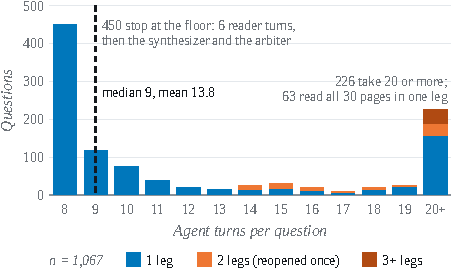
\includegraphics[width=\columnwidth]{appendix/figures/method_trajectory.pdf}
\caption{Agent turns per question on MMLongBench-Doc, by the number of reading cycles. A cycle is the \texttt{reader}'s turns followed by one \texttt{synthesizer} and one \texttt{arbiter} turn.}
\label{fig:app_trajectory}
\end{figure}

% \begin{figure}[t]
% \centering
% \includegraphics[width=\columnwidth]{appendix/figures/method_trajectory_ldu.pdf}
% \caption{Agent turns per question on LongDocURL, by the number of reading cycles.}
% \label{fig:app_trajectory_ldu}
% \end{figure}

\paragraph{Reading Depth.}
The system does not uniformly consume its page budget (Figure~\ref{fig:app_trajectory}). Of the 1,067 questions it finished, 450 end after eight agent turns, the earliest point the reading floor $k=6$ permits: six \texttt{reader} turns, one \texttt{synthesizer} turn, and one \texttt{arbiter} turn. Progressively fewer questions read deeper, and 226 take twenty turns or more, including 63 that read all $B=30$ pages in a single cycle. Reopened trajectories, in which the \texttt{arbiter} requests further reading, account for part of this tail. The median question reads 7 pages, well beyond the one or two gold pages that most answerable questions cite. That gap reflects the deployed setting: the locations of the evidence pages are unknown, so coverage has to be bought with reading depth.
% On LongDocURL, ... (Figure~\ref{fig:app_trajectory_ldu}).
